%%%%%%%%%%%%%%%%%%%%%%%%%%%%%%%%%%%%%%%%%
% Thesis 
% LaTeX Template
% Version 1.3 (21/12/12)
%
% This template has been downloaded from:
% http://www.latextemplates.com
%
% Original authors:
% Steven Gunn 
% http://users.ecs.soton.ac.uk/srg/softwaretools/document/templates/
% and
% Sunil Patel
% http://www.sunilpatel.co.uk/thesis-template/
%
% License:
% CC BY-NC-SA 3.0 (http://creativecommons.org/licenses/by-nc-sa/3.0/)
%
% Note:
% Make sure to edit document variables in the Thesis.cls file
%
%%%%%%%%%%%%%%%%%%%%%%%%%%%%%%%%%%%%%%%%%

%----------------------------------------------------------------------------------------
%	PACKAGES AND OTHER DOCUMENT CONFIGURATIONS
%----------------------------------------------------------------------------------------

\documentclass[11pt, a4paper, oneside]{Thesis} % Paper size, default font size and one-sided paper
\usepackage[utf8]{inputenc}
\graphicspath{{./FIGS/}} % Specifies the directory where pictures are stored


% MY PACKAGES
\usepackage{algorithm, algorithmic}



\usepackage[square, comma, sort&compress]{natbib} % Use the natbib reference package - read up on this to edit the reference style; if you want text (e.g. Smith et al., 2012) for the in-text references (instead of numbers), remove 'numbers' 
\hypersetup{urlcolor=blue, colorlinks=true} % Colors hyperlinks in blue - change to black if annoying
\title{\ttitle} % Defines the thesis title - don't touch this

\begin{document}

\frontmatter % Use roman page numbering style (i, ii, iii, iv...) for the pre-content pages

\setstretch{1.3} % Line spacing of 1.3

% Define the page headers using the FancyHdr package and set up for one-sided printing
\fancyhead{} % Clears all page headers and footers
\rhead{\thepage} % Sets the right side header to show the page number
\lhead{} % Clears the left side page header

\pagestyle{fancy} % Finally, use the "fancy" page style to implement the FancyHdr headers

\newcommand{\HRule}{\rule{\linewidth}{0.5mm}} % New command to make the lines in the title page

% PDF meta-data
\hypersetup{pdftitle={\ttitle}}
\hypersetup{pdfsubject=\subjectname}
\hypersetup{pdfauthor=\authornames}
\hypersetup{pdfkeywords=\keywordnames}
\newcommand{\ra}[1]{\renewcommand{\arraystretch}{#1}}

%----------------------------------------------------------------------------------------
%	QUOTATION PAGE
%----------------------------------------------------------------------------------------

\pagestyle{empty} % No headers or footers for the following pages

\null\vfill % Add some space to move the quote down the page a bit

\textit{``Thanks to my solid academic training, today I can write hundreds of words on virtually any topic without possessing a shred of information, which is how I got a good job in journalism."}

\begin{flushright}
Dave Barry
\end{flushright}

\vfill\vfill\vfill\vfill\vfill\vfill\null % Add some space at the bottom to position the quote just right

\clearpage % Start a new page

%----------------------------------------------------------------------------------------
%	ACKNOWLEDGEMENTS
%----------------------------------------------------------------------------------------

\setstretch{1.3} % Reset the line-spacing to 1.3 for body text (if it has changed)

\acknowledgements{\addtocontents{toc}{\vspace{1em}} % Add a gap in the Contents, for aesthetics

The acknowledgements and the people to thank go here, don't forget to include your project advisor\ldots
}
\clearpage % Start a new page

%----------------------------------------------------------------------------------------
%	LIST OF CONTENTS/FIGURES/TABLES PAGES
%----------------------------------------------------------------------------------------

\pagestyle{fancy} % The page style headers have been "empty" all this time, now use the "fancy" headers as defined before to bring them back

\lhead{\emph{Contents}} % Set the left side page header to "Contents"
\tableofcontents % Write out the Table of Contents

\lhead{\emph{List of Figures}} % Set the left side page header to "List of Figures"
\listoffigures % Write out the List of Figures

\lhead{\emph{List of Tables}} % Set the left side page header to "List of Tables"
\listoftables % Write out the List of Tables

%----------------------------------------------------------------------------------------
%	ABBREVIATIONS
%----------------------------------------------------------------------------------------

\clearpage % Start a new page

\setstretch{1.5} % Set the line spacing to 1.5, this makes the following tables easier to read

\lhead{\emph{Abbreviations}} % Set the left side page header to "Abbreviations"
\listofsymbols{ll} % Include a list of Abbreviations (a table of two columns)
{
\textbf{LAH} & \textbf{L}ist \textbf{A}bbreviations \textbf{H}ere \\
%\textbf{Acronym} & \textbf{W}hat (it) \textbf{S}tands \textbf{F}or \\
}

%----------------------------------------------------------------------------------------
%	PHYSICAL CONSTANTS/OTHER DEFINITIONS
%----------------------------------------------------------------------------------------

\clearpage % Start a new page

\lhead{\emph{Physical Constants}} % Set the left side page header to "Physical Constants"

\listofconstants{lrcl} % Include a list of Physical Constants (a four column table)
{
Speed of Light & $c$ & $=$ & $2.997\ 924\ 58\times10^{8}\ \mbox{ms}^{-\mbox{s}}$ (exact)\\
% Constant Name & Symbol & = & Constant Value (with units) \\
}

%----------------------------------------------------------------------------------------
%	SYMBOLS
%----------------------------------------------------------------------------------------

\clearpage % Start a new page

\lhead{\emph{Symbols}} % Set the left side page header to "Symbols"

\listofnomenclature{lll} % Include a list of Symbols (a three column table)
{
$a$ & distance & m \\
$P$ & power & W (Js$^{-1}$) \\
% Symbol & Name & Unit \\

& & \\ % Gap to separate the Roman symbols from the Greek

$\omega$ & angular frequency & rads$^{-1}$ \\
% Symbol & Name & Unit \\
}

%----------------------------------------------------------------------------------------
%	DEDICATION
%----------------------------------------------------------------------------------------

\setstretch{1.3} % Return the line spacing back to 1.3

\pagestyle{empty} % Page style needs to be empty for this page

\dedicatory{For/Dedicated to/To my\ldots} % Dedication text

\addtocontents{toc}{\vspace{2em}} % Add a gap in the Contents, for aesthetics

%----------------------------------------------------------------------------------------
%	THESIS CONTENT - CHAPTERS
%----------------------------------------------------------------------------------------

\mainmatter % Begin numeric (1,2,3...) page numbering

\pagestyle{fancy} % Return the page headers back to the "fancy" style

% # Flow around contra-rotating open rotors: general information
%     * Background
%     * Aerodynamic of an isolated propeller
%     * Aerodynamic of a contra-rotating open rotor
%     * A few words on aeroelasticity
%         - experimental aeroelasticity
%         - numerical aeroelasticity
% 
% # Generalities
%     * equation that I solve
%     * elsA
%     * ALE / aeroelasticity presentation
%!TEX root = ../main.tex
\chapter{Generalities}
\label{generalities}

\lhead{Chapitre ??. \emph{Generalities}}

\section{Equation solved} % (fold)
\label{sec:equation_solved}

The Unsteady Reynolds-Averaged Navier-Stokes (U-RANS) equations in
integral form are given by
\begin{equation}
   \int_\Omega \frac{\partial W}{\partial t} dV + \oint_{\partial
     \Omega} \overrightarrow{F} \cdot \overrightarrow{N} ds = 0,
   \label{eq:intNS}
\end{equation} 
where $\overrightarrow{F}$~is the flux across $\partial \Omega$ and
$W$~is the vector of the conservative unknowns (conservative variables
and turbulent variables).  Assuming $\Omega$ is a
control volume, the semi-discrete finite-volume form of the
U-RANS equations is obtained from Eq.~\eqref{eq:intNS}:
\begin{equation}
   \frac{d}{dt} \left(V  \overline{W}\right) + R \left( \overline{W}
   \right) = 0,
   \label{eq:semiDiscNS}
\end{equation} 
with $V$~the volume of the cell~$\Omega$, $R$~the residual resulting
from the discretization of the fluxes and the source terms (including
the turbulent equations), and $\overline{W}$ the mean of the
unknowns over the control volume.  In the following, the over line
symbol~$\overline{\cdot}$ is dropped out for clarity.

\section{Fluid / Structure Interaction}

\subsection{Weak Coupling Approach}

The weak coupling approach~\cite{Rougeault2003} is a one way
  coupling from structure to fluid: First, a modal identification
of the structure is carried out. Then the fluid response to the
harmonic prescribed motion of the structure modes is simulated,
where the harmonic motion of the geometry is ensured by a mesh
deformation technique, based on a structural analogy method
implementing linear elastic elements. Finally, knowing the unsteady
pressure load, a stability study can be performed in the frequency
domain.

\subsection{Linear Modal Structure Model}

\subsubsection{Governing Equations}
Once the modal basis $\Phi$ is identified, either by mean of a Finite
Element model or an experimental identification, the equation of
structure dynamics under aerodynamic load $F_A$ reads:
\begin{equation}
  \label{eq:2}
  M\ddot{q}+D\dot{q}+Kq-\Phi^\top F_A(t)=0, \quad x=\Phi q.
\end{equation}
The weak coupling approach assumes the linearity of the response of
the fluid with respect to the displacement of the structure. Therefore
small displacements are assumed and the so-called Generalized
Aerodynamic Forces (GAF) are linearized, which adds aerodynamic
stiffness~$K_A$ and damping~$D_A$:
\begin{equation}
  \label{eq:4}
  \Phi^\top F_A(t) = D_A\dot{q}+K_Aq.
\end{equation}
In order to estimate the unsteady aerodynamic forces $F_A(t)$,
  a fluid simulation is run with a prescribed harmonic motion of the
  structure:
\begin{equation}
  \label{eq:6}
  q(t)=\cos(\omega t).
\end{equation}
A stability analysis is then performed in the frequency domain:
\begin{equation}
  \label{eq:5}
  q=\hat{q}e^{p t}\Rightarrow\left(
    p^2M + p(D-D_A) + (K-K_A)
  \right)\hat{q}=0,
\end{equation}
where the Laplace variable $p$ is of the form
$p=i\omega(1+i\alpha)$. Finally, considering only weakly damped or
amplified modes (i.e. $|\alpha| \ll 1$), the damping of the
fluid/structure coupled system reads $\alpha=-\Re e(p)/\Im m(p)$.

\subsubsection{Single Passage Reduction for Turbomachinery Computations}

As the blade row is rotating, the stiffness of the blades is increased
and gyroscopic terms are added. Equation~\eqref{eq:2} becomes
\begin{equation}
  \label{eq:gyr}
  M\ddot{q}+(D+D_G)\dot{q}+(K+K_G)q-\Phi^\top F_A(t)=0, \quad x=\Phi q,
\end{equation}
where $D_G$ is the skew-symmetric gyroscopic damping matrix and $K_G$ is
the gyroscopic matrix of deflection for inclusion of centrifugal
elements for instance.  The disk being flexible, the blades do not vibrate
independently of each other. The cyclic symmetry leads to complex
vibration modes, which can be seen as rotating waves traveling at an
integer multiple $n_d$ of the rotation speed \cite{Lane:1956fk}. $n_d$
is called a nodal diameter. Opposite nodal diameters have the same
vibration mode propagating in opposite directions. Therefore their
respective modes are complex conjugate.


% section aeroelasticity_module (end)

% section equation_solved (end)

% 
% # Harmonic balance methods
%     * state of the art
%         - Numeca
%         - Duke
%         - He
%     * mono-frequential
%         - theory
%         - advantages
%         - applications that can be treated
%     * multi-frequential (advantages and questions that it raises)
%         - theory
%         - advantages
%         - applications that can be treated
% 
% # Validation
%     * toy problems (advantages)
%         - capturing a sinusoidal flow
%         - capturing a wake / clocking effects
%     * toy problems (drawbacks)
%         - non evenly spaced timelevels
%         - signal to capture (wake / sinus / step function)
% 
% # Improving the method
%     * algorithm to automatically choose the timelevels
%!TEX root = ../main.tex

%     * convergence of spectral methods : analyzing the spectrum of the wake
%     * partial conclusion: we may go to industrial applications
% 
% # application to the aeroelasticity of contra-rotating open rotors
%     * validation of the proposed approach (STCF 11)
%!TEX root = ../main.tex
\chapter{Application to the aeroelasticity of contra-rotation open rotors} % (fold)
\label{cha:application_to_the_aeroelasticity_of_contra_rotation_open_rotors}

\lhead{Chapitre ??. \emph{Application to the aeroelasticity of CRORs}}

\section{Validation of the proposed approach} % (fold)
\label{sec:validation_of_the_proposed_approach}


For external-flow aeroelasticity, the HB approach has 
been thoroughly validated~\cite{Gopinath2005,Sicot2008,Woodgate2009,Dufour2010}, 
mostly for the AGARD test cases of Davis~\cite{Davis1982}. 
However, experimental data for turbomachinery aeroelasticity are more scarce: 
the Standard Aeroelastic Configurations experiments 
of Fransson~\textit{et al.}~\cite{Fransson:1999uq} are the 
reference in this respect, and have been widely used 
to validate different numerical approaches~\cite{Sbardella:2001fk,
Duta:2002uq,Campobasso:2003fk,Cinnella2004,mcbean2005}. 


The $11$\textsuperscript{th} standard configuration is a
turbine stator composed of 20~blades, and tested at EPF-Lausanne
in the late 1990's by Fransson~\emph{et al.}~\cite{Fransson:1999uq}.
The test cascade is placed in a 
annular test rig as depicted in~Fig.\ref{fig:annular_channel}
\begin{figure}[htbp]
  \centering
  \includegraphics*[width=0.40\textwidth]{./ANNULAR_CHANNEL.pdf}
  \caption{Annular test rig for the standard configurations}
  \label{fig:annular_channel}
\end{figure}
The experimental results have been found to be highly reproducible and
therefore suitable for code validation~\cite{Fransson:1999uq}.  


% geometry presentation
The geometry profile and the results are available over the
internet~\cite{stcf11web}.  To allow local validation of the steady
flow, the isentropic Mach number is given at blade wall.

The blades oscillate harmonically in the first bending mode
at a reduced frequency of $f_{c} =\pi \cdot c \cdot
f/U_{outlet, exp} = 0.2134$ for the subsonic case and $0.1549$ for the
transonic case. Aeroelastic
results are available such as the first harmonic of the unsteady pressure
coefficient at blade walls (amplitude and phase), for several nodal
diameters. The integrated
results, such as the damping, strongly vary under small changes in the
local distribution. It is therefore recommended to look at the local
distributions.
 
% mesh presentation
The blade passage is meshed using an O4H topology (Fig.~\ref{fig:stcf11_mesh}).  
The number of grid points along the blade
chord axis is~160 and the computed $y^+$ at the walls is $\mathcal{O}(1)$. % proving
The blade has the same profile along the spanwise direction and no
twist. Therefore, a 2.5D mesh is used with five points in the radial direction, with a spanwise
extent representing $1\%$ of the chord. 

% boundary conditions
The boundary conditions used for this case are: (i)~an
injection condition  for the inlet (with a relative flow angle
set to the  experimental value), (ii)~a constant static pressure
condition for the outlet,  (iii)~an adiabatic no-slip condition on
blade walls, and (iv)~periodic or phase-lagged conditions for azimuthal boundaries depending on the  
prescribed IBPA.

% numerical parameters
Turbulence is modeled using the one-equation model of
Spalart-Allmaras~\cite{Spalart1992}.  The third-order upwind Roe
scheme~\cite{Roe1981} is used to compute the convective fluxes.
The maximum
CFL number is set to~20 for the steady computations,  the inner loop
of the DTS scheme and the HB simulations.  For the DTS scheme,  
convergence in time discretization is obtained
after 20~periods using 128~instants per period.  Iterative convergence 
for the inner loop is considered achieved when the normalized
residuals drop by $5\cdot 10^{-2}$ (within a maximum of
50~sub-iterations).

\subsection{Subsonic Case}
The measured inlet Mach number is $0.31$ and the isentropic outlet Mach number is $0.69$.
% steady results
Steady results for the isentropic Mach number at blade walls are compared to the experimental data in 
Fig.~\ref{fig:stcf11_rans_subsonic}.  For this flow regime, the flow
remains subsonic.
On the pressure side, the flow accelerates all the way
to the trailing edge of the blade. On the suction side, the flow
accelerates until a maximum speed at $\approx 40~\%$ of the chord and
then decelerates (Fig.~\ref{fig:stcf11_subsonic_field_mis_bw}).
The agreement with the experimental data is fair. However, an
over-prediction of the isentropic Mach number is observed on the suction
side.  This discrepancy is also reported in the literature (see
Ref.~\cite{Fransson:1999uq} for instance).
\begin{figure}[htb]
  \centering
  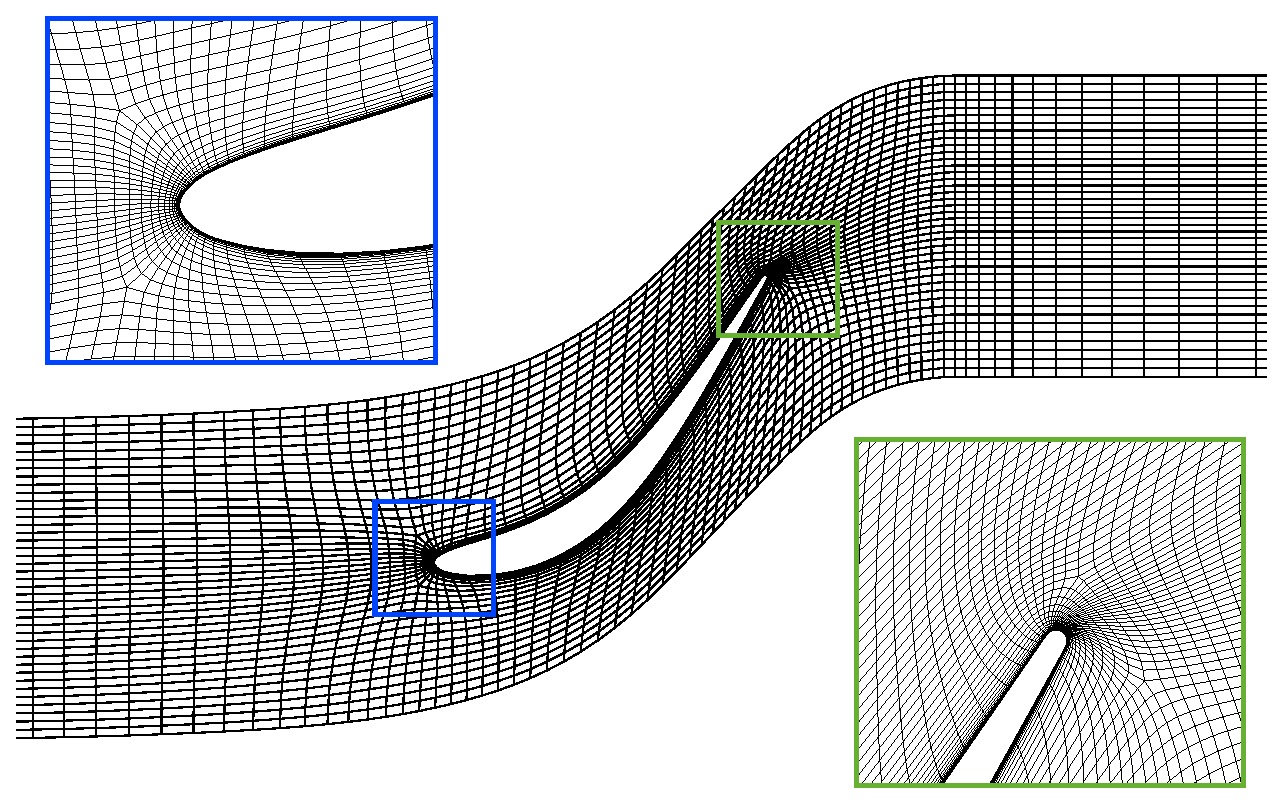
\includegraphics[width=.46\linewidth]{STCF11_MESH.eps}
  \caption{STCF 11 mesh}
  \label{fig:stcf11_mesh}
\end{figure}

\begin{figure}[htb]
  \centering
  \begin{minipage}[b]{.46\linewidth}
    \centering
    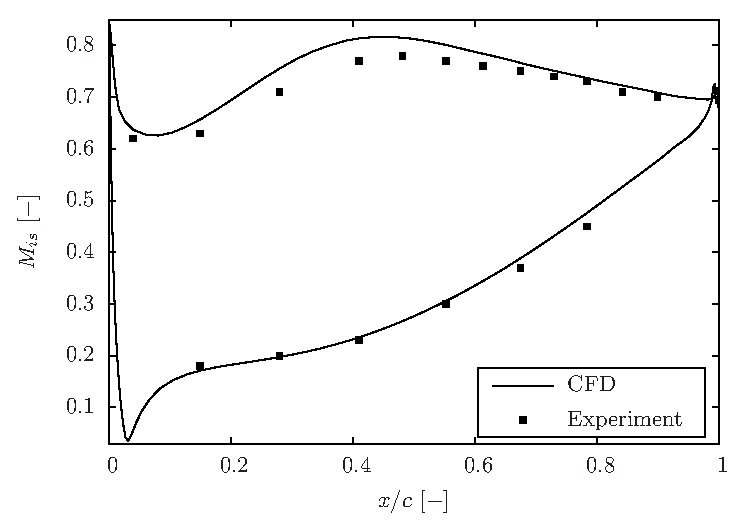
\includegraphics[width=\textwidth]{STCF11_RANS_SUBSONIC.eps}
    \caption{Steady results of the isentropic Mach number at blade
      walls, subsonic case}
    \label{fig:stcf11_rans_subsonic}
  \end{minipage}\quad
  \begin{minipage}[b]{.46\linewidth}
    \centering
    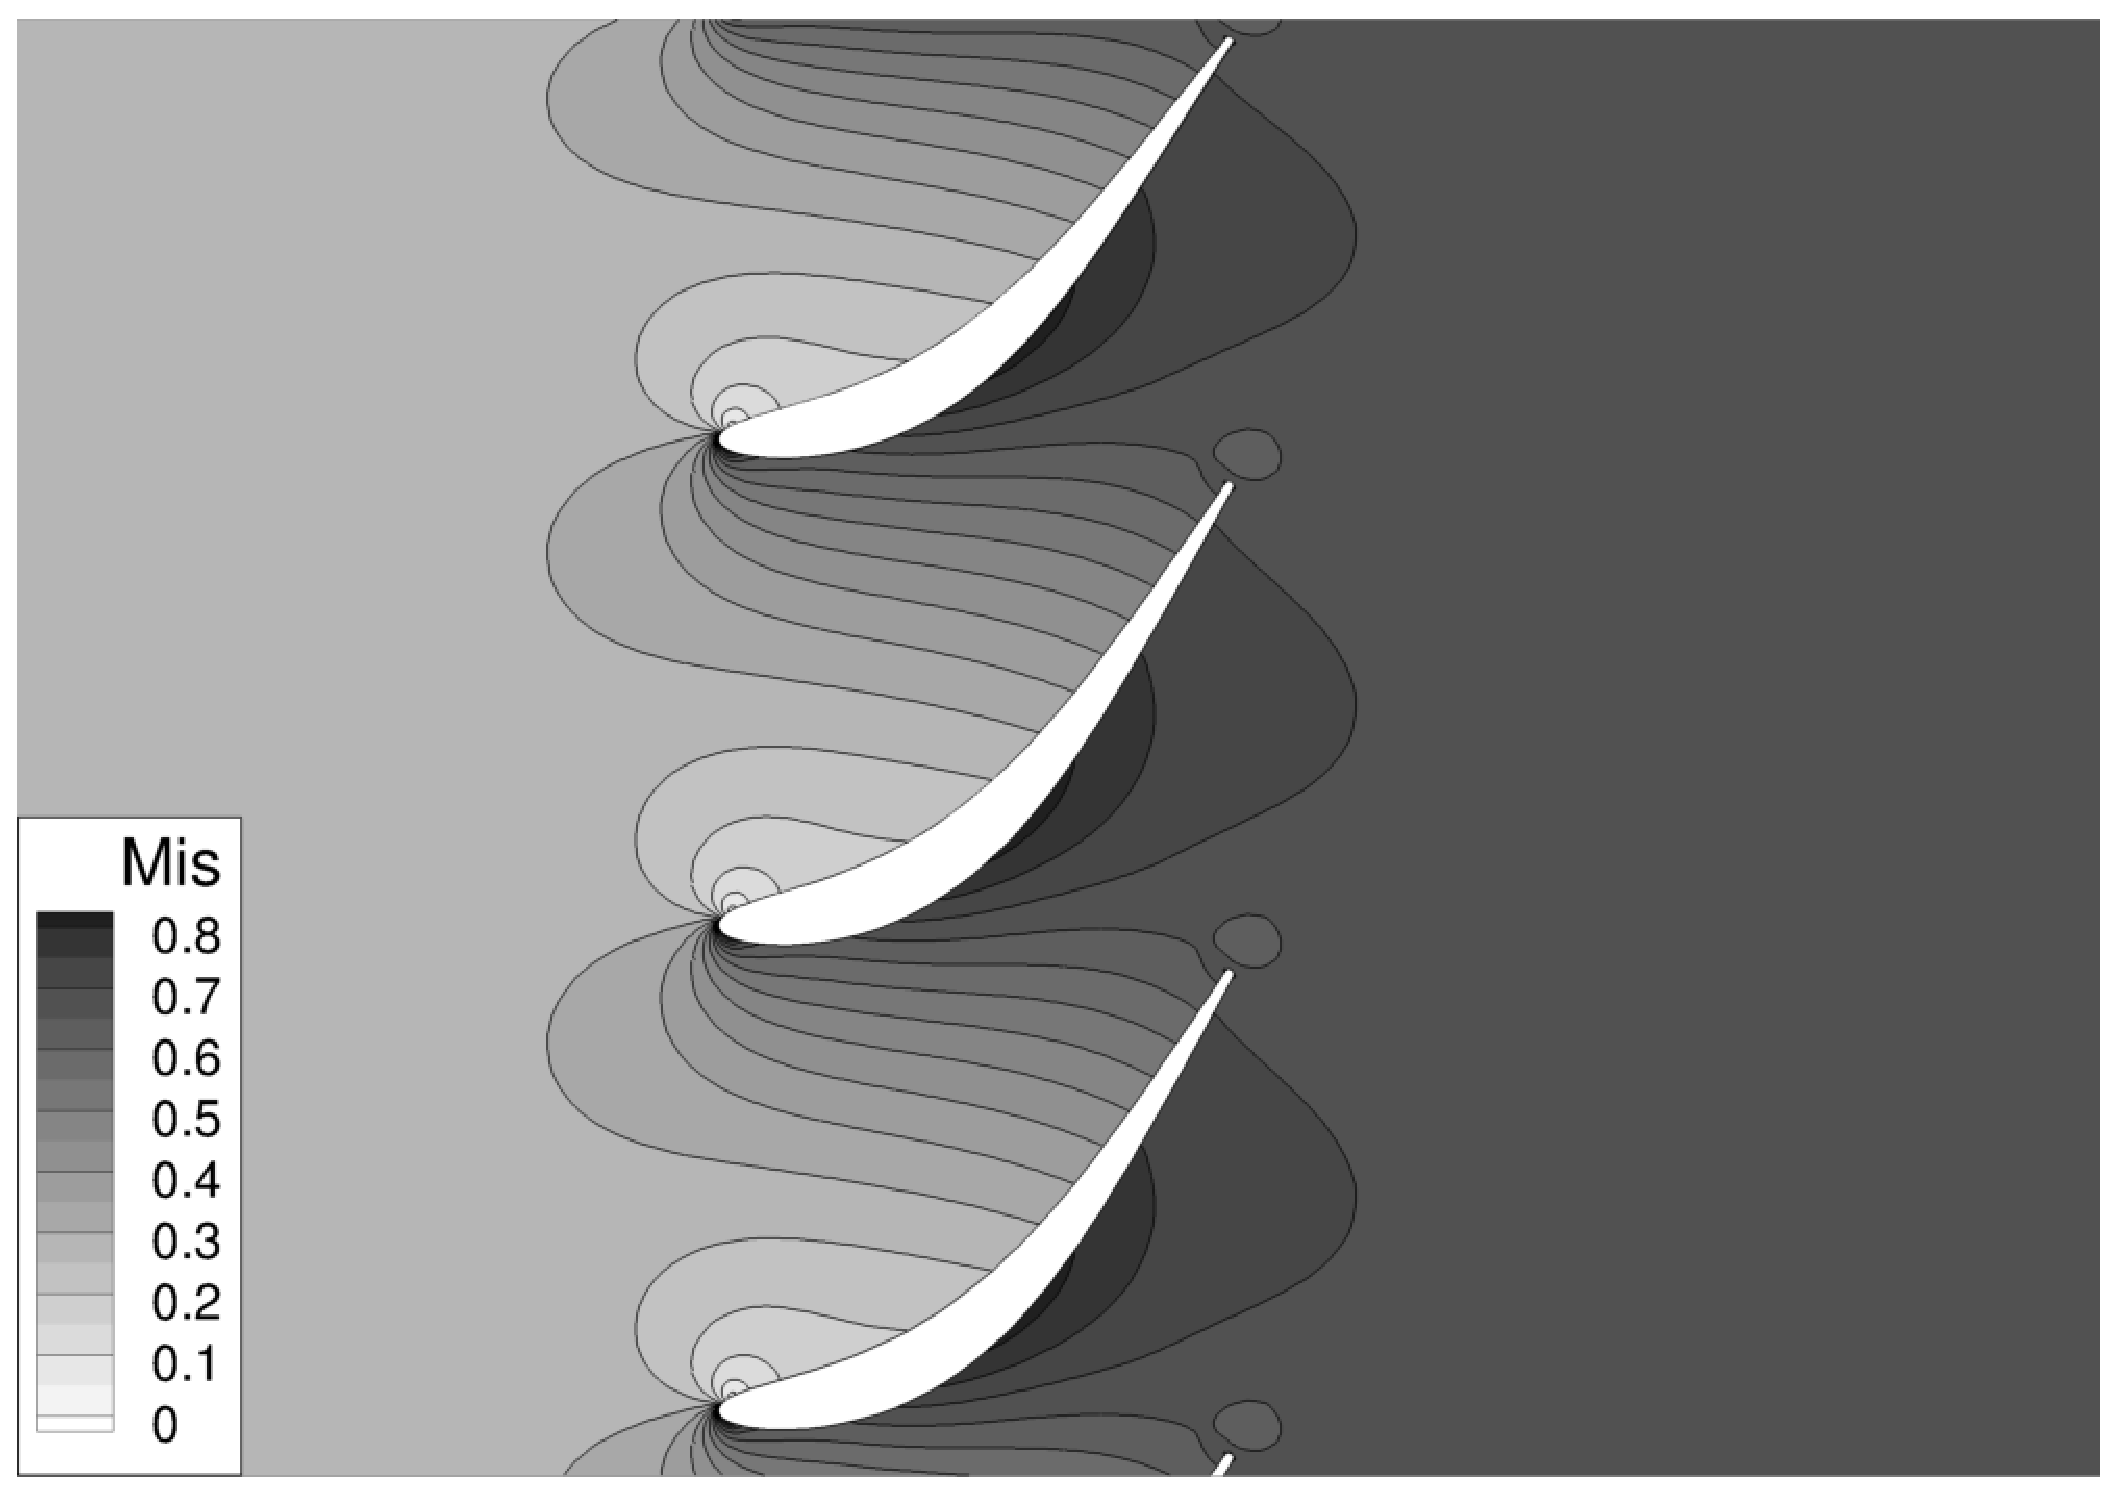
\includegraphics[width=\textwidth]{STCF11_SUBSONIC_FIELD_MIS_BW.eps}
    \caption{Steady isentropic Mach number contours, subsonic case}
    \label{fig:stcf11_subsonic_field_mis_bw}
  \end{minipage}
\end{figure}

% unsteady results
The aeroelastic experimental data are compared to the present results
obtained with both the DTS and the HB approach. To explore the range
of nodal diameters with the HB method, an incremental approach is used
where each nodal diameter simulation is used to initialize the next
one.  Considering the opposite phase vibration case (the 10\textsuperscript{th} nodal diameter), 
the amplitude and the phase of the pressure coefficient are
presented in Fig.~\ref{fig:stcf11_ael_subsonic_ibpa_180_paper}.
With only one harmonic (\emph{i.e.},~three instants), the HB results
are superimposed on the DTS ones. Moreover, the numerical results are
in fair agreement with the experimental data for the
amplitude. However, for the phase, the sign change on the
suction side is predicted at about $60~\%$ of the chord, whereas the
experimental location is about 25~\%.
\begin{figure}[htb]
  \centering 
  \begin{tabular}{cc}
    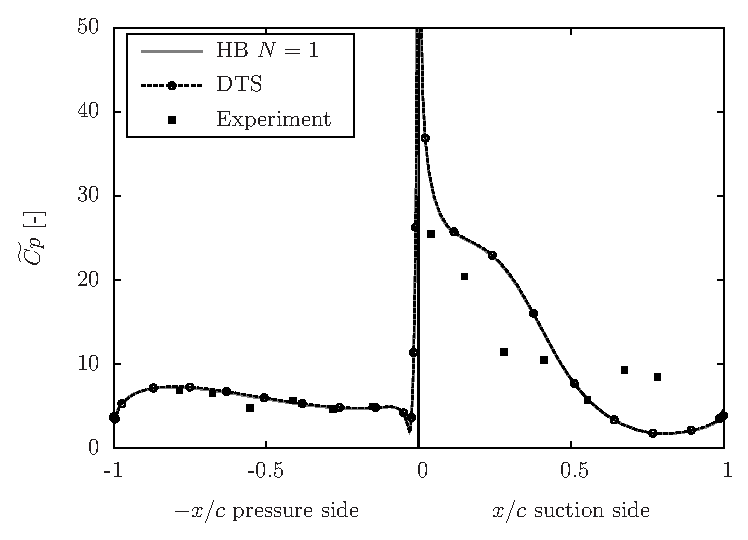
\includegraphics[width=.45\textwidth]{STCF11_AEL_SUBSONIC_IBPA_180_Cp_paper.eps}
    &
    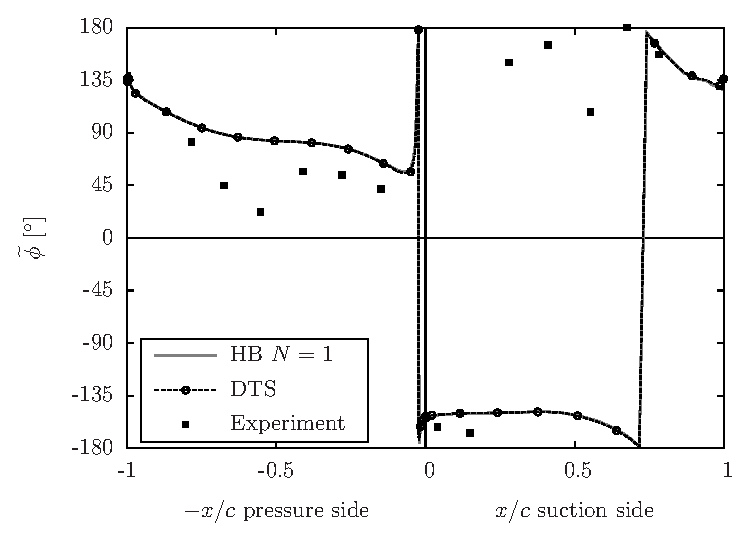
\includegraphics[width=.45\textwidth]{STCF11_AEL_SUBSONIC_IBPA_180_Phi_paper.eps}\\
    (a) Amplitude part & (b) Phase part
  \end{tabular}
  \caption{Wall pressure harmonic analysis for an opposite phase vibration, subsonic case}
  \label{fig:stcf11_ael_subsonic_ibpa_180_paper}
\end{figure}


The results for the  nodal  diameter $-2$ are shown
in Fig.~\ref{fig:stcf11_ael_subsonic_ibpa_324_paper}. The HB and DTS data
are superimposed, and are in fair agreement with the experiments. The
amplitude levels are well captured and the phase prediction is
slightly improved over the opposite phase case.
\begin{figure}[htb]
  \centering 
  \begin{tabular}{cc}
    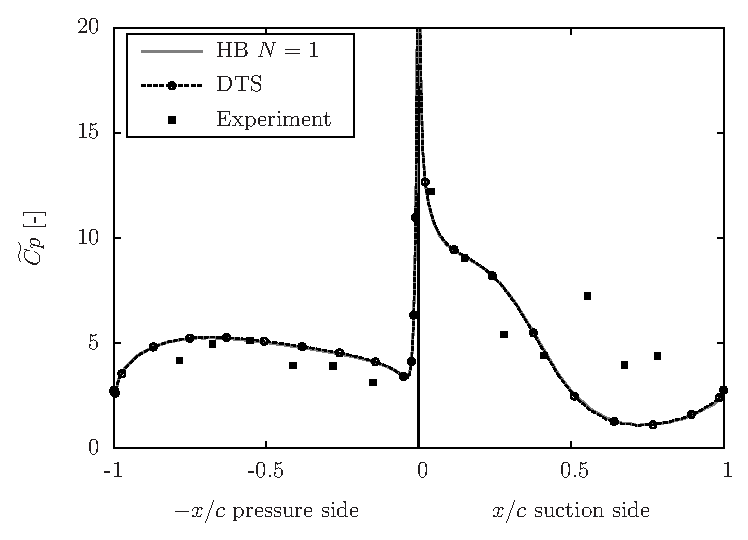
\includegraphics[width=.45\textwidth]{STCF11_AEL_SUBSONIC_IBPA_324_Cp_paper.eps}
    &
    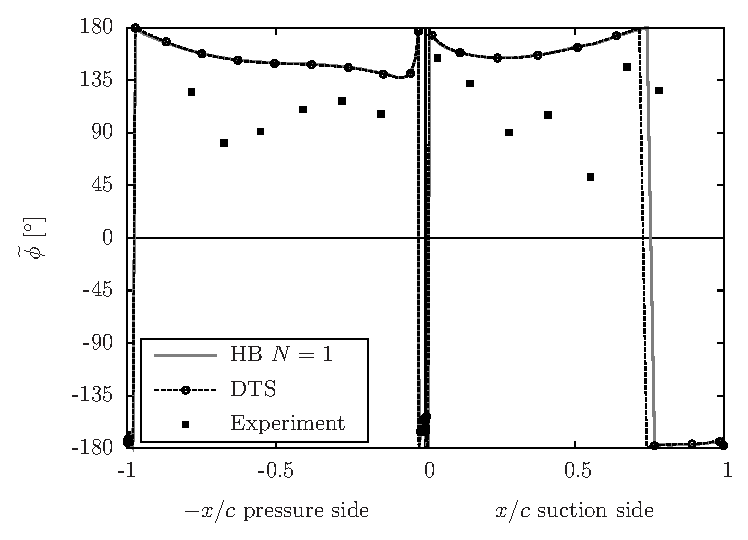
\includegraphics[width=.45\textwidth]{STCF11_AEL_SUBSONIC_IBPA_324_Phi_paper.eps}\\
    (a) Amplitude part & Phase part
  \end{tabular}
  \caption{Wall pressure harmonic analysis for \mbox{$n_d=-2$}, subsonic case}
  \label{fig:stcf11_ael_subsonic_ibpa_324_paper}
\end{figure}

The damping obtained from the previous calculations is depicted 
in Fig.~\ref{fig:stcf11_subsonic_damping}.  Also plotted are the results
from Fransson~\emph{et al.}~\cite{Fransson:1999uq}, obtained with both
potential, linear Euler, non-linear Euler and non-linear viscous codes.
The results for all IBPAs are given for the potential code but only $\beta=180^\circ$ is provided for the other codes~\cite{Fransson:1999uq}.
These are the only damping results for the
subsonic case known by the authors.  Since the local variations are
superimposed for the DTS and the HB approaches, so are the damping.
The present
results show similar trends and levels to those of Fransson~\emph{et al.} 
\begin{figure}[htb]
  \centering
  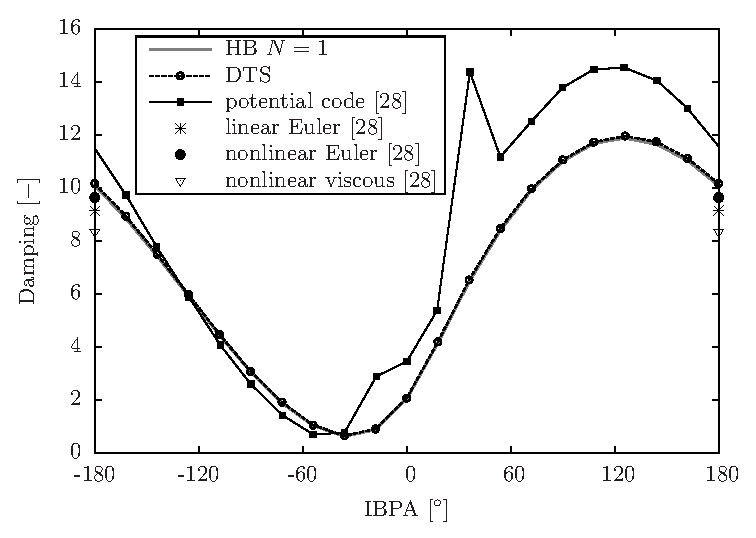
\includegraphics[width=.46\linewidth]{STCF11_SUBSONIC_DAMPING.eps}
  \caption{Aerodynamic damping coefficient versus IBPA, subsonic case}
  \label{fig:stcf11_subsonic_damping}
\end{figure}



\subsection{Transonic Condition}
The outlet isentropic Mach number is $0.99$ for an inlet Mach number of $0.4$. 
This case, for which experimental uncertainties are available, 
has been largely addressed in the literature 
(see for instance Refs.~\cite{Sbardella:2001fk,Duta:2002uq,Campobasso:2003fk,Cinnella2004}). 
This test case is challenging in terms of nonlinearities as a separation bubble and a shock are present.

Steady results of the isentropic Mach number are shown in
Fig.~\ref{fig:stcf11_rans_transonic}.  For this flow regime,
a small separation
bubble develops on the suction side at the leading edge~(cf.~Fig.~\ref{fig:stcf11_transonic_field_mis_bw}).  The flow then accelerates, followed by a passage shock.  
The experimental data suggests that the shock appears
sooner on the suction side than in the computations; all the results 
reported in the literature exhibit similar discrepancies (see
Refs.~\cite{Fransson:1999uq,Sbardella:2001fk,Duta:2002uq,Campobasso:2003fk,Cinnella2004}). 
Otherwise, the present results are in fair agreement with experimental data.
\begin{figure}[htb]
  \centering
  \begin{minipage}[b]{.46\linewidth}
    \centering
    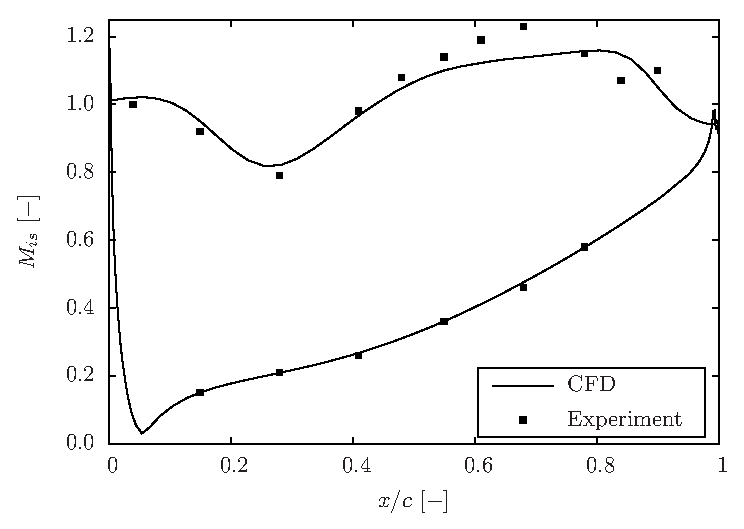
\includegraphics[width=\textwidth]{STCF11_RANS_TRANSONIC.eps}
    \caption{Steady results of the isentropic Mach number at blade
      wall, transonic case}
    \label{fig:stcf11_rans_transonic}
  \end{minipage}\quad
  \begin{minipage}[b]{.46\linewidth}
    \centering
    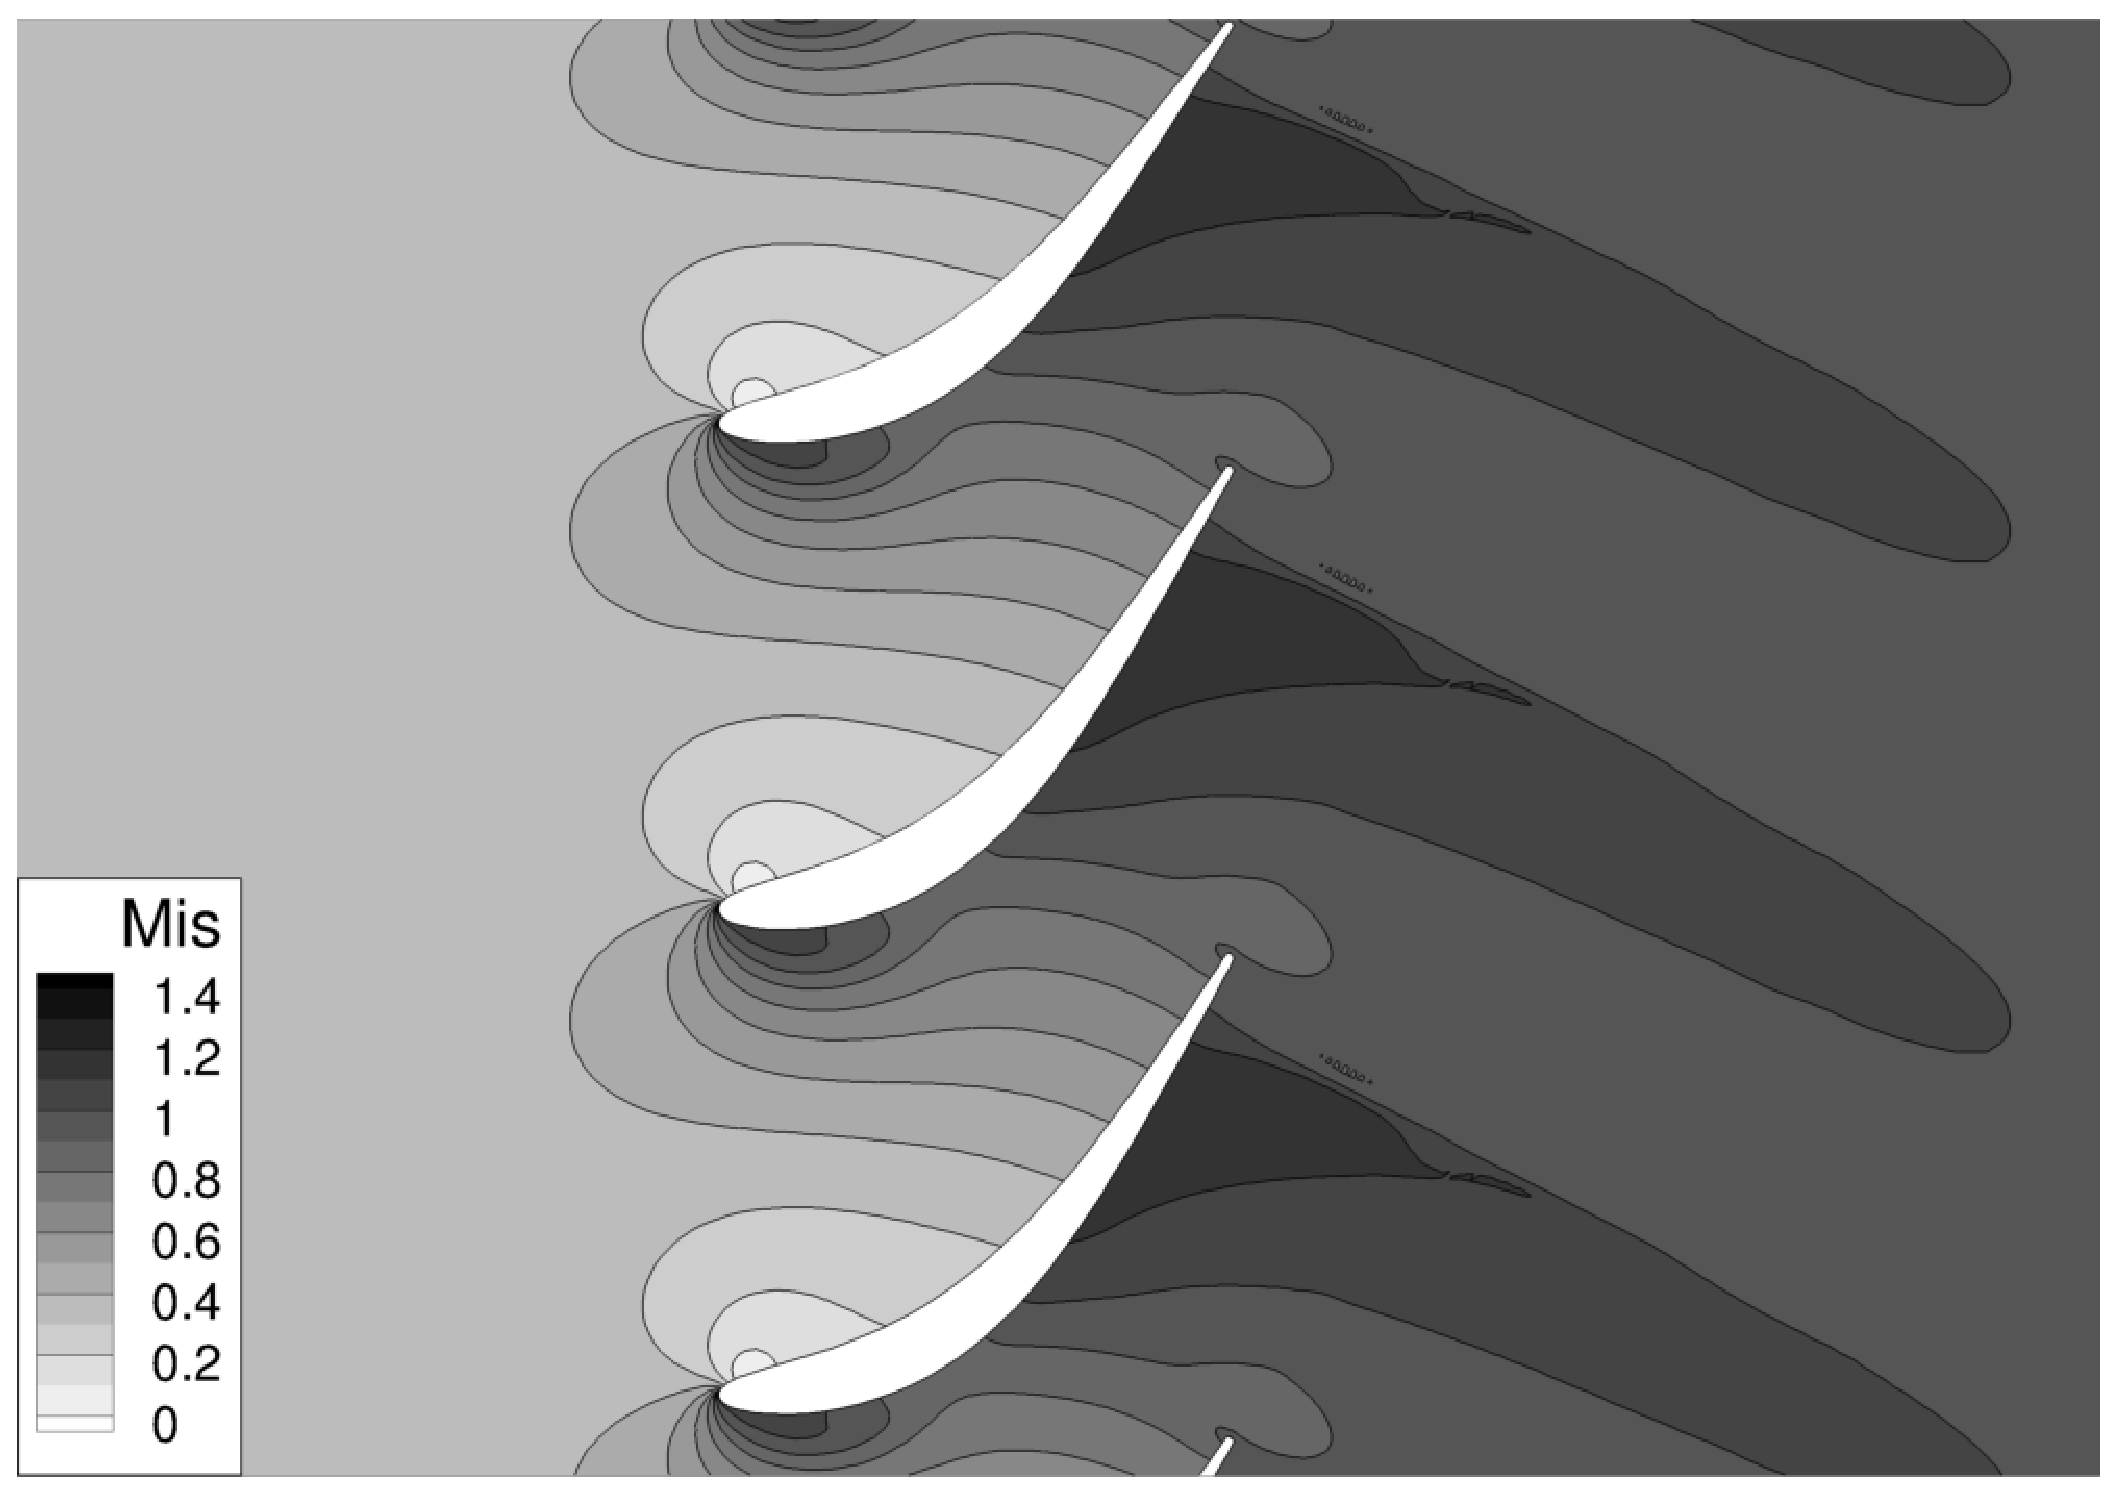
\includegraphics[width=\textwidth]{STCF11_TRANSONIC_FIELD_MIS_BW.eps}
    \caption{Steady isentropic Mach number contours, transonic case}
    \label{fig:stcf11_transonic_field_mis_bw}
  \end{minipage}
\end{figure}

% unsteady results
The aeroelastic experimental data are compared to the present results
obtained with both the DTS and the HB approach.  Considering the opposite phase vibration case (the 10\textsuperscript{th} nodal diameter), 
the amplitude and the
phase of the pressure coefficient are presented in
Fig.~\ref{fig:stcf11_ael_transonic_ibpa_180_paper}. Also plotted are the results of
Cinnella~\emph{et~al.}~\cite{Cinnella2004}, computed with a nonlinear viscous
approach using the Spalart-Allmaras turbulence model. The present HB and the DTS
results are superimposed, which indicates that the one harmonic HB solution is able
to reproduce the unsteady nonlinear effects without increasing the
number of harmonics. This observation is only valid near the wall,
before the harmonics are created naturally by the flow, due to the
nonlinear effects. The results are in good agreement with
the experimental data and display the same trends as that of
Cinnella~\emph{et~al.}  A slight discrepancy can be observed within the shock
region, where the amplitude and the phase phenomena are predicted
further than the experiments indicate.  This can be attributed to the poor
prediction of the shock position and hence the poor prediction
of its interaction with the motion of the blade.
\begin{figure}[htb]
  \centering
  \begin{tabular}{cc}
    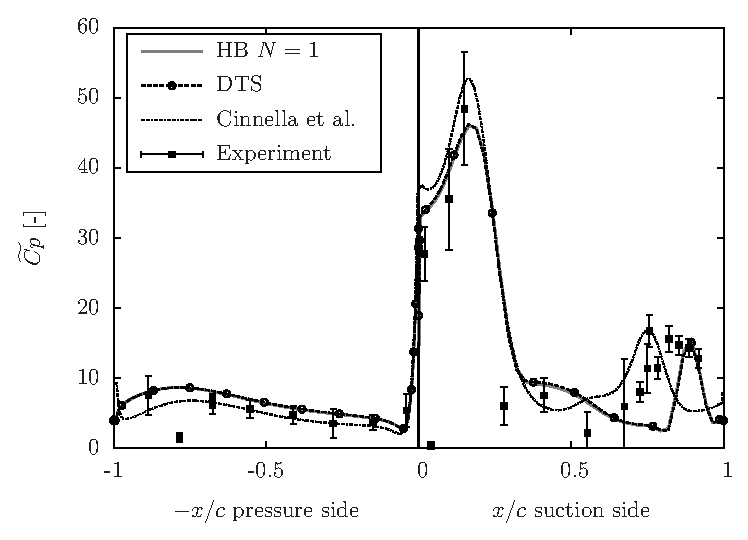
\includegraphics[width=.45\textwidth]{STCF11_AEL_TRANSONIC_IBPA_180_Cp_paper.eps}
    &
    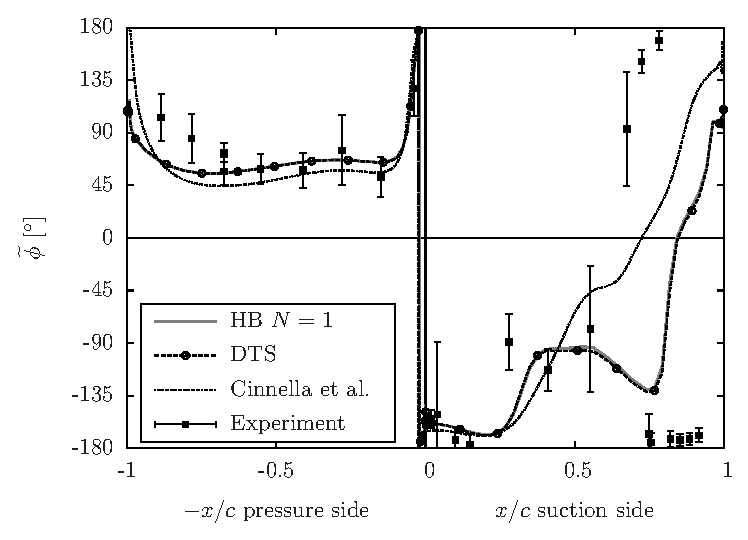
\includegraphics[width=.45\textwidth]{STCF11_AEL_TRANSONIC_IBPA_180_Phi_paper.eps}\\
    (a) Amplitude part & Phase part
  \end{tabular}
  \caption{Wall pressure harmonic analysis for an opposite phase vibration, transonic case}
  \label{fig:stcf11_ael_transonic_ibpa_180_paper}
\end{figure}

The results for the $-2$\textsuperscript{th} nodal diameter are also shown in
Fig.~\ref{fig:stcf11_ael_transonic_ibpa_324_paper}. Again,
the HB results are superimposed on the DTS ones. Moreover, these are in
good agreement with the experiments, considering the uncertainties of
the experimental data.
\begin{figure}[htb]
  \centering 
  \begin{tabular}{cc}
    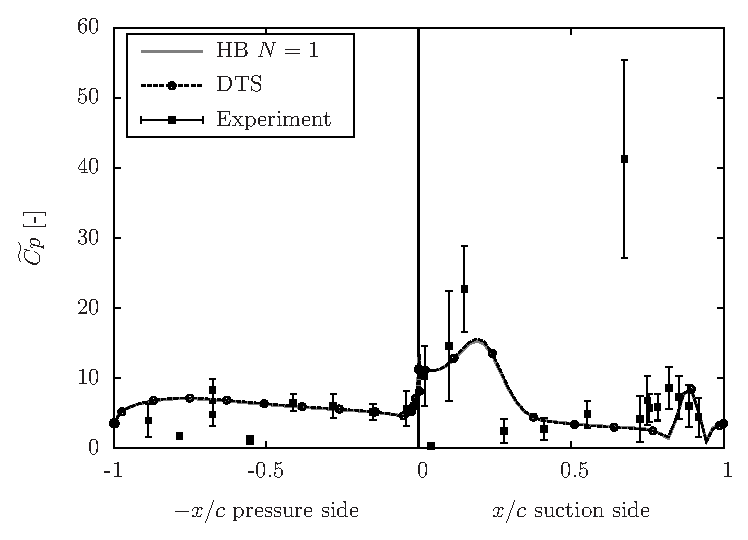
\includegraphics[width=.45\textwidth]{STCF11_AEL_TRANSONIC_IBPA_324_Cp_paper.eps}
    &
    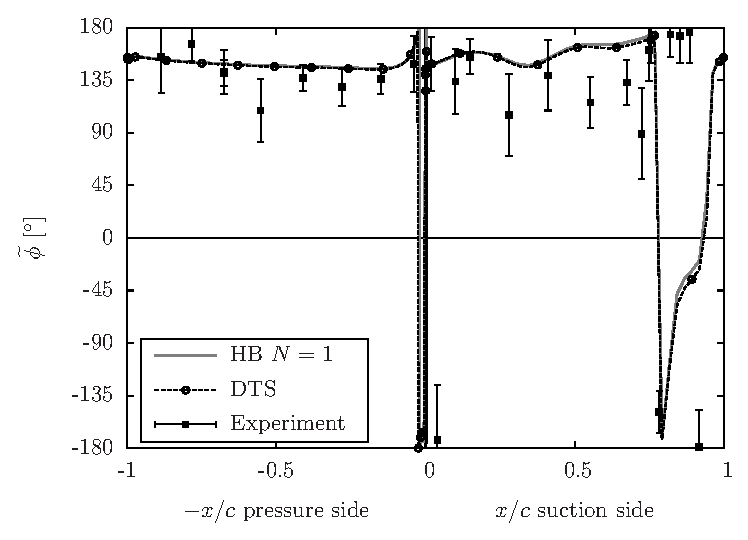
\includegraphics[width=.45\textwidth]{STCF11_AEL_TRANSONIC_IBPA_324_Phi_paper.eps}\\
    (a) Amplitude part & (b) Phase part
  \end{tabular}
  \caption{Wall pressure harmonic analysis for \mbox{$n_d=-2$}, transonic case}
  \label{fig:stcf11_ael_transonic_ibpa_324_paper}
\end{figure}

The damping is shown in Fig.~\ref{fig:stcf11_transonic_damping} for
the transonic case. Also plotted are the results from
Fransson~\emph{et al.} (potential code), and 
from Cinnella~\emph{et al.} (RANS). The scattering is much more severe
than for the subsonic case. The trends obtained with the RANS approaches are similar. However, the
discrepancies between the two RANS codes are significant in terms of
levels.
Recently, Vogt and Fransson~\cite{Vogt:2011fk} reported similar discrepancies 
for damping predictions of subsonic and transonic cascades, 
showing that the damping can be significantly affected by 
small local changes in the amplitude and/or the phase.
\begin{figure}[htb]
  \centering
  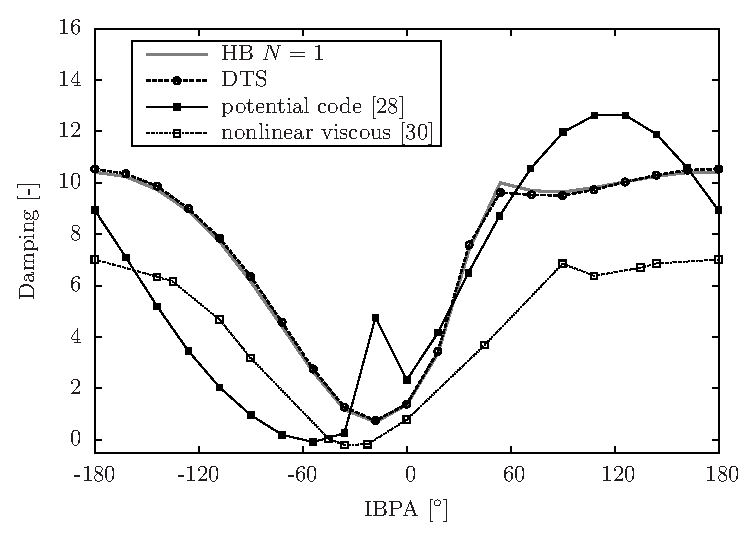
\includegraphics[width=.46\linewidth]{STCF11_TRANSONIC_DAMPING.eps}
  \caption{Aerodynamic damping coefficient versus IBPA, transonic
    case}
  \label{fig:stcf11_transonic_damping}
\end{figure}
In terms of computational efficiency, the HB method is 7 times faster
than the DTS  for all the IBPAs.

% section validation_of_the_proposed_approach (end)

% chapter application_to_the_aeroelasticity_of_contra_rotation_open_rotors (end)

%     * aeroelasticity of an isolated contra-rotating open rotor
%     * aeroelasticity of an installed contra-rotating open rotor


%----------------------------------------------------------------------------------------
%	THESIS CONTENT - APPENDICES
%----------------------------------------------------------------------------------------

\addtocontents{toc}{\vspace{2em}} % Add a gap in the Contents, for aesthetics

\appendix % Cue to tell LaTeX that the following 'chapters' are Appendices

% Include the appendices of the thesis as separate files from the Appendices folder
% Uncomment the lines as you write the Appendices

%!TEX root = ../main.tex
\chapter{Validation of the convection code}
\label{Appendix_convection_code}

%\input{./Appendices/AppendixB}
%\input{./Appendices/AppendixC}

\addtocontents{toc}{\vspace{2em}} % Add a gap in the Contents, for aesthetics

\backmatter

%----------------------------------------------------------------------------------------
%	BIBLIOGRAPHY
%----------------------------------------------------------------------------------------

\label{Bibliography}

\lhead{\emph{Bibliography}} % Change the page header to say "Bibliography"

\bibliographystyle{unsrtnat} % Use the "unsrtnat" BibTeX style for formatting the Bibliography

\bibliography{biblio} % The references (bibliography) information are stored in the file named "Bibliography.bib"

\end{document}  